Having defined the classical system we wish to study, we use standard numerical practices to obtain the time evolution of Matrix theory observables. The details of the numerical methods can be found in \cref{app:numerical-methods}.

\begin{figure}[H]
    \centering
    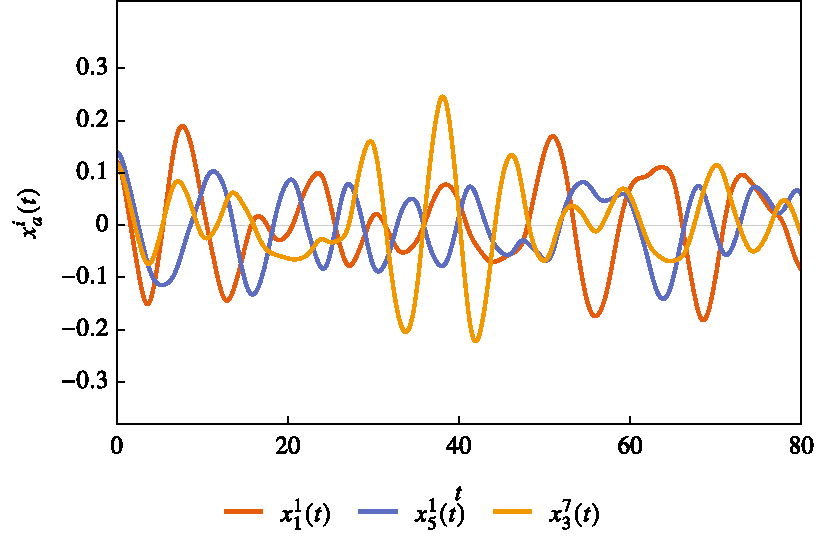
\includegraphics{1-elements}
    \caption{Numerical simulation of a few matrix coefficients starting with random initial conditions of the kind described in \cref{app:numerical-methods} for $N = 9$}
    \label{fig:1-elements}
\end{figure}

We restrict our attention to initial conditions of a specific type. Namely, those with zero initial velocities
\begin{equation}
    \dot{X}^{i}(0) = 0
\end{equation}

This has two benefits:
\begin{enumerate}
    \item[a.] {The Gauss constraint%
    \begin{equation}
        \comm{X^i}{\dot{X}^i} = 0
    \end{equation}%
    is automatically satisfied at $t = 0$. Moreover, since the constraint is a constant of motion (as always with gauge constraints), time evolution (if done correctly) guarantees that the constraint will always be satisfied.}
    \item[b.] {The $\mathrm{SO}(9)$ angular momentum%
    \begin{equation}
        \mathcal{J}^{i j} = \Tr \left( X^{i} \dot{X}^{j} - X^{j} \dot{X}^{i} \right)
    \end{equation}%
    which is also a conserved charge, vanishes at all times. In other words, we are looking at the zero angular momentum sector of BFSS, and there are good reasons to do so \cite{Chowdhury:2015gbk}.}
\end{enumerate}

The initial "positions" $X^{i}(0)$ are taken to be random Hermitian matrices (see \cref{app:numerical-methods}), and we study many such random states for different sizes of matrices $N$. The time evolution of a typical such state (or rather, of its coefficients in an $\mathfrak{su}(N)$ basis) looks as in \cref{fig:1-elements}


\begin{figure}[H]
    \centering
    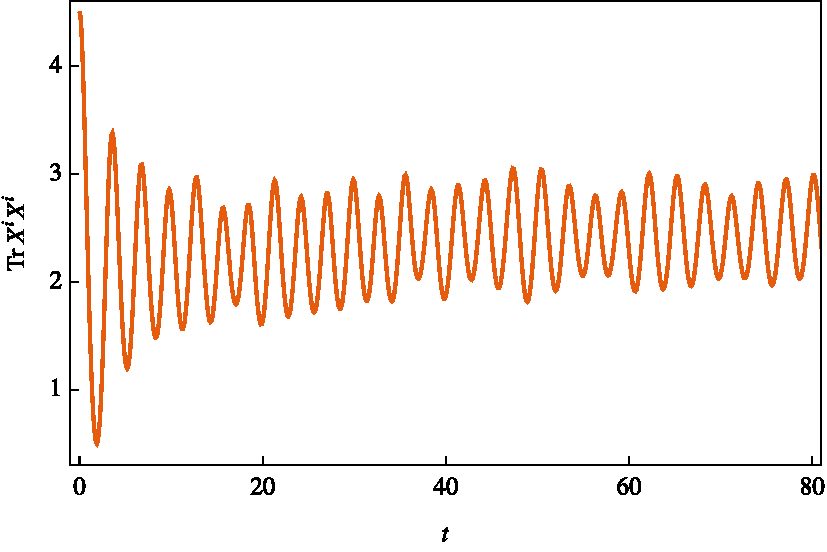
\includegraphics{1-trX2}
    \caption{Dynamics of the simplest gauge and rotational invariant operator $\Tr X^i X^i$ for the state in \cref{fig:1-elements}}
    \label{fig:1-trX2}
\end{figure}


\section{Horizon Dynamics}

When the BFSS Matrix model has a tractable classical supergravity dual, the black brane solution has a horizon whose radius $r_0$ can be related to the observable $\Tr X^i X^i$ in the matrix model.
\begin{equation}
    r_0 \sim \sqrt{\frac{1}{N} \Tr X^i X^i}
\end{equation}

\begin{figure}[H]
    \centering
    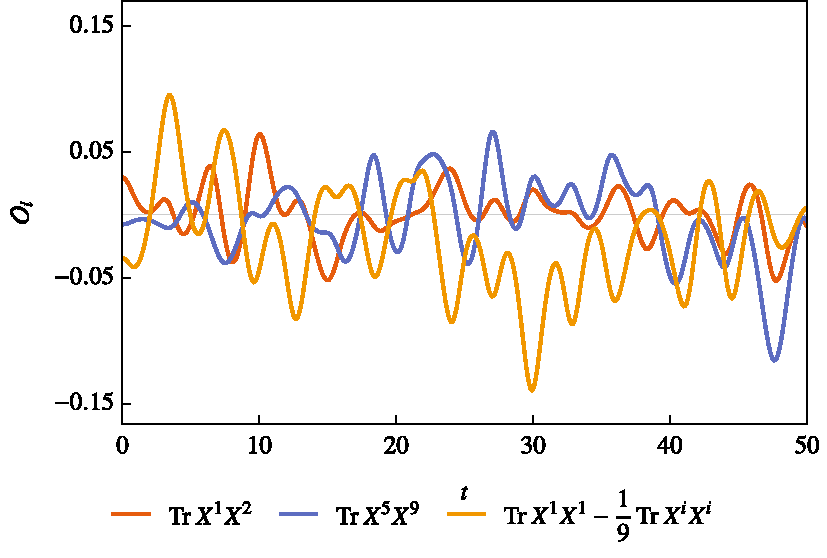
\includegraphics{3-quadrupole}
    \caption{Few components of the symmetric traceless tensor $\mathfrak{S}^{i j}$ for the state in \cref{fig:1-elements}}
    \label{fig:3-quadrupole}
\end{figure}

Therefore, one expects that the time evolution of $\Tr X^i X^i$ captures the microscopic dynamics of the black hole horizon in the underlying geometry. For the state in \cref{fig:1-elements}, the corresponding dynamics of $\Tr X^i X^i$ is shown in \cref{fig:1-trX2}

Other interesting observables can be constructed from single trace higher order polynomials in the $X$s. In supergravity, these can be interpreted as higher order multipoles, deviations from $\mathrm{SO}(9)$ spherical invariance. The simplest one is the symmetric traceless $\mathrm{SO}(9)$ tensor
\begin{equation}\label{eqn:symm-trace-tensor}
    \mathfrak{S}^{i j} = \Tr \left( X^i X^j \right) - \frac{\delta^{i j}}{K} \Tr \left( X^k X^k \right)
\end{equation}
along with other higher-order observables, such as
\begin{align}
    \mathfrak{C}_{(3a)}^{i} &= \Tr \left( X^{i} X^j X^{j} \right) \\
    \mathfrak{C}_{(3b)}^{i j k} &= \Tr \left( X^{(i} X^j X^{k)} \right) \\
    \mathfrak{Q}_{(4a)} &= \Tr \left( X^i X^j X^i X^j \right) \\
    \mathfrak{Q}_{(4b)} &= \Tr \left( X^i X^j X^j X^i \right)
\end{align}
A few components of $\mathfrak{S}^{i j}$ and $\mathfrak{Q}_{(4a)}$ are shown for the state in \cref{fig:1-elements} in \cref{fig:3-quadrupole}, and \cref{fig:3-trXiXjXiXj}

\begin{figure}[H]
    \centering
    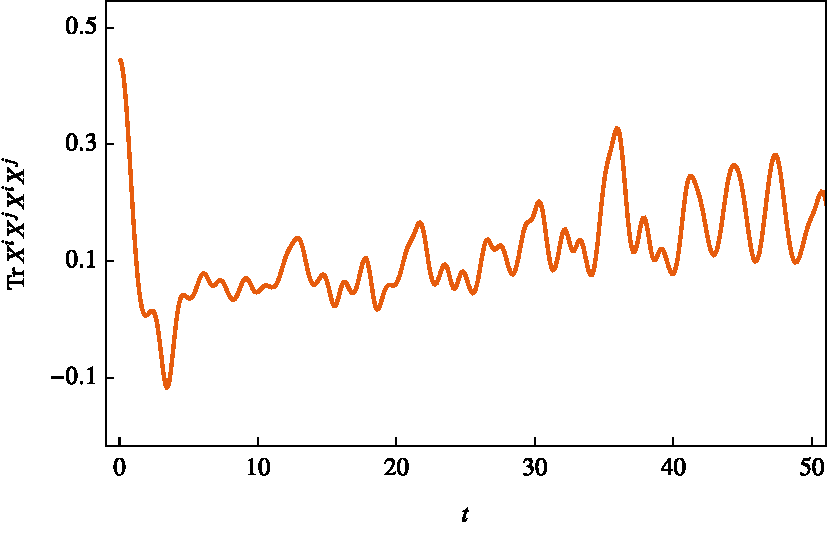
\includegraphics{3-trXiXjXiXj}
    \caption{One of the two quartic observables $\mathfrak{Q}_{(4a)}$. Note that it forms one-half of the bosonic potential of BFSS}
    \label{fig:3-trXiXjXiXj}
\end{figure}

\section{Sensitivity to initial conditions}
The bosonic model under consideration exhibits sensitivity to initial conditions. One can see this explicitly by considering two random initial states that differ by a small amount $\epsilon$. To achieve this, generate two initial conditions $X_{(\text{orig})}$ and $X_{(2)}$ in the manner demonstrated in \cref{app:numerical-methods} and define
\begin{equation}
    X_{(\text{pert})} = X_{(\text{orig})} + \epsilon X_{(2)}
\end{equation}
where the matrix and $\mathrm{SO}(9)$ vector indices have been supressed. The result of numerically evolving these states for $\epsilon = 10^{-6}$ is given in \cref{fig:2-chaos}. Not that the two trajectories for the matrix elements and the gauge invariant observable $\Tr X^i X^i$ diverge at slightly different times.

One can quantify this dependence on initial conditions by considering an appropriate gauge invariant distance between the two states. One way is to define it as
\begin{equation}
    \label{eqn:dist-two-states}
    R^2 = \sum_{i} \Tr \left( X^i_{(\text{pert})} - X^i_{(\text{orig})} \right)^2
\end{equation}
One can go even further and do this for an entire cloud of initial conditions. Suppose we start with $m$ initial conditions $X_{(a)} \ (a = 1,\ldots,m)$ that are $\epsilon$ away from each other in the manner described above. The average location of these states is
\begin{equation}
    Z^i = \frac{1}{m} \sum_{a} X^{i}_{(a)}
\end{equation}

\begin{figure}[H]
    \centering
    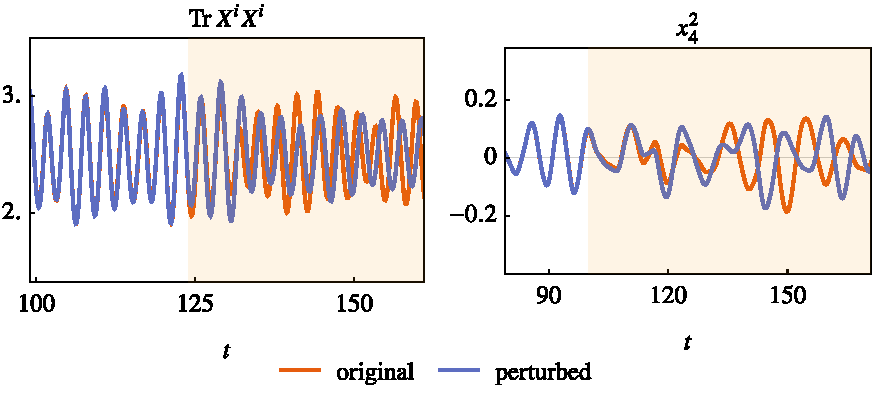
\includegraphics{2-chaos}
    \caption{A demonstration of chaos in the classical dynamics. Both plots show the dynamics of two states that start very close to each other $\epsilon \sim 10^{-6}$ but eventually diverge.}
    \label{fig:2-chaos}

    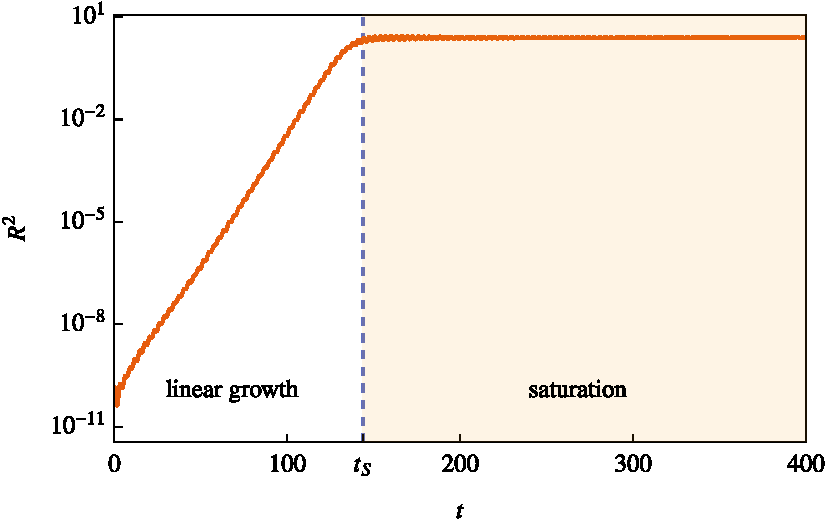
\includegraphics{2-saturation}
    \caption{A log-scale plot of the spread of states in phase space $R^2$ as a function of time. Note the two phases: linear growth followed by saturation}
    \label{fig:2-saturation}
\end{figure}

A straightforward generalization of \cref{eqn:dist-two-states} is
\begin{equation}
    R^2 = \frac{1}{m} \sum_{a, i} \Tr \left( X^i_{(a)} - Z^i \right)^2
\end{equation}

A plot of $R^2$ starting at $m = 48$ initial conditions close to each other within $\epsilon = 10^{-6}$ is shown in \cref{fig:2-saturation}. Remarkably, one observes two well-separated regions of time, best seen on a log scale. The distance measure starts growing linearly, as expected in a typical chaotic system. It does this until a time $t_S$, around which it settles down into an almost constant value. This saturation region extends to arbitrarily long times, and we shall call $t_S$ the \textit{saturation time}.


This feature of an initial regime of linear growth followed by saturation is observed universally at all points on the phase space and for all values of the parameters under consideration: matrix size $N$, number of matrices $K$, and the number of initial conditions $m$.

One way to visualize this is to take three-dimensional sections of the entire phase space and observe the trajectories of the various states. One finds precisely as one expects: the trajectories start in a tiny dense ball (of size $\sim\epsilon$) and initially evolve as a single state at the location of the ball would. However, the ball grows as it evolves until it gets big enough to fill a sizable portion of phase space. Around $t = t_S$, the ball stops growing, but the various points that make up this gas of states start jiggling around endlessly while maintaining its approximate shape and size.

So far, we have discovered a dynamical time scale: the saturation time $t_S$. Later when we look at statistics of various observables over long times, it would be helpful to exclude the initial region of linear growth and compute statistics from, say, $t = 200 > t_S$ to $t = T$ where we take $T$ to be of the order of $1000$ or $10,000$.

\begin{figure}[H]
    \centering
    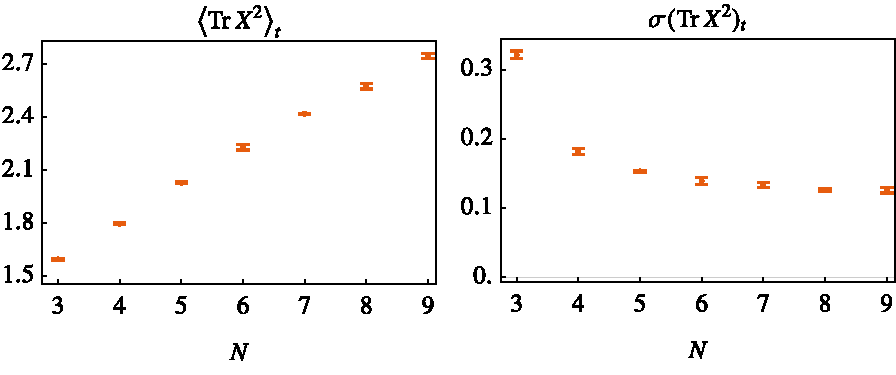
\includegraphics{4-monopole}
    \caption{The time average (left) and standard deviation (right) of $\Tr X^2$ for many states of normalized energy $E = 1$ as a function of matrix size $N$. The error bars indicate the dependence of the statistic on the chosen initial condition.}
    \label{fig:4-monopole}
\end{figure}

\section{Memorlylessness}

Upon looking at \cref{fig:2-saturation}, it is very tempting to suggest that even though the precise dynamical evolution of states is highly initial condition dependent, the overall features, such as long-time averages of various observables might lose such dependence on the initial state. If this is the case, due to the scaling similarity of \cref{eqn:scaling-similarity}, one would expect long time averages of observables homogenous in the $X$s to only depend on the energy of the energy surface being explored. This dependence follows easily from the scaling relations \cref{eqn:scaling-similarity}.

The most straightforward check for solution independence is to compute the long-time averages (and higher statistics) of various observables. This is done in \cref{fig:4-monopole} for $\Tr X^i X^i$ and in \cref{fig:4-quadrupole} for the symmetric traceless tensor $\mathfrak{S}^{i j}$ of \cref{eqn:symm-trace-tensor} for different matrix sizes. The error bars in the figures indicate how much the corresponding statistic changes for different initial conditions of the same energy.

From these figures, it seems that certain observables like $\Tr X^i X^i$ exhibit universal behavior at long times more than others, even though the trend indicates that perhaps more and more higher-order observables start to "thermalize" (obtain stable time averages) as we go to larger values of $N$. 




\begin{figure}[H]
    \centering
    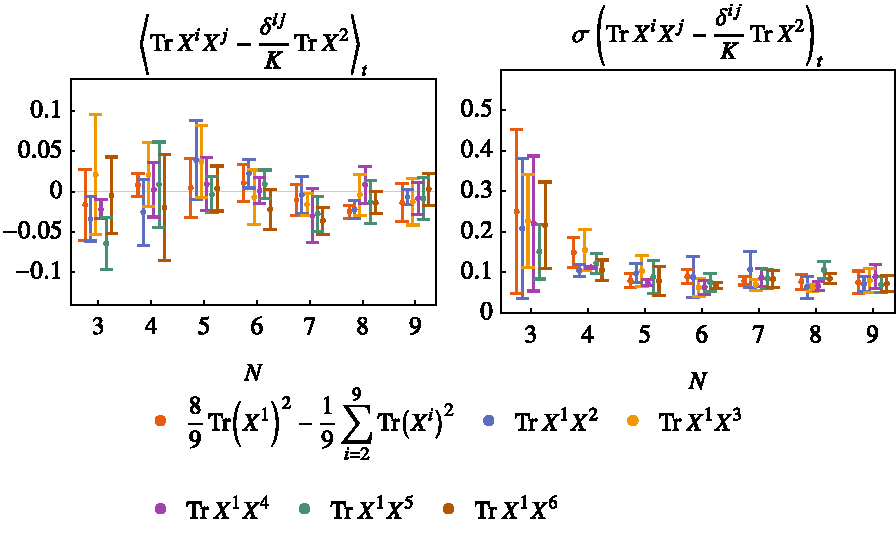
\includegraphics{4-quadrupole}
    \caption{Time statistics for a few components of the symmetric traceless tensor $\mathfrak{S}^{i j}$.}
    \label{fig:4-quadrupole}
\end{figure}

Random matrix theory suggests that a critical observable in any matrix model is the set of eigenvalues of the matrices. In \cref{fig:6-eig-sol-indep}, we plot the (time) distribution of the eigenvalues of the various $X^i$. We do not specify which $X^i$ because these distributions look more or less exactly the same (up to numerical inaccuracies) for different matrices $X^i$. The plots show this distribution arising from two different initial conditions, (a) and (b). The almost perfect overlap between them is more evidence to support memorlylessness.

For those familiar with random matrix distributions, \cref{fig:6-eig-sol-indep} would appear a familiar pattern. Indeed, this is qualitatively, the shape of the distribution of eigenvalues for a Gaussian Unitary Ensemble (GUE). This observation will be explored further in the next section.

\begin{figure}[H]
    \centering
    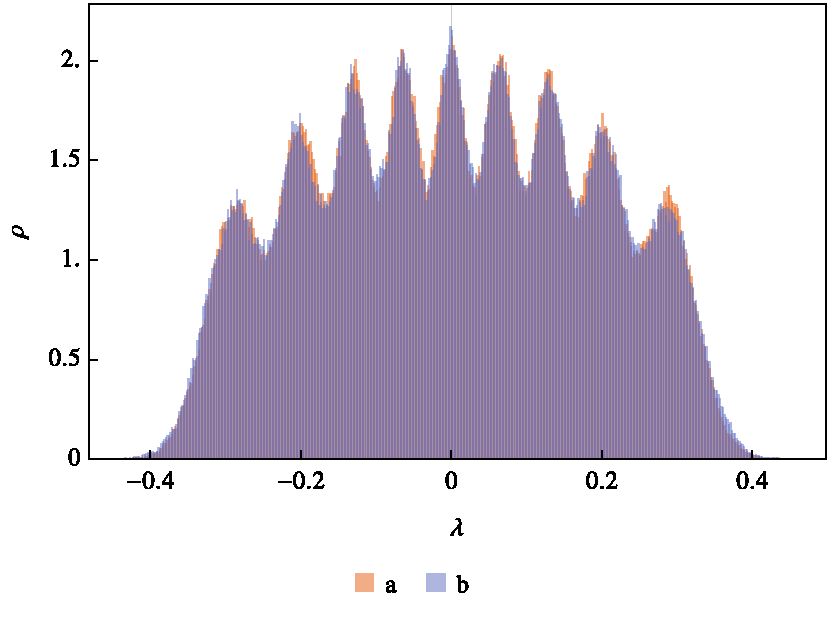
\includegraphics{6-eig-sol-indep}
    \caption{The eigenvalue (time) distribution for $N = 9$ starting at two random initial states (a) and (b). Note that all eigenvalues (of all matrices $X^i$) have been clubbed together since they have identical distributions.}
    \label{fig:6-eig-sol-indep}
\end{figure}

Lastly, one can also look at the full distribution of $\Tr X^i X^i$. This is shown in \cref{fig:6-solution-independence}. The overlap, in this case, is not as good as the eigenvalues but is satisfactory enough to take memorlylessness as a feature of the bosonic model we are studying seriously.  

\section{Connections to random matrices}
We will not explore in greater detail the observation that the eigenvalue distribution arising from the time evolution of the matrix eigenvalues looks suspiciously close to a Gaussian random matrix distribution of Hermitian matrices.

Perhaps the most preliminary question in this regard is the covariance matrix $\mathrm{Cov}(X^i, X^j)$ or equivalently, in a suitable $\mathfrak{su}(N)$ basis, the object
\begin{equation}
    c_{i a, j b} = \mathrm{Cov} \left( x^i_a , x^j_b \right)
\end{equation}
Since each matrix has $N^2 - 1$ components and there are $K$ of them, this is a $(K(N^2-1)) \times (K(N^2-1))$ real symmetric matrix. For $K = 9, N = 9$, $K(N^2-1) = 720$. Evaluating this matrix is a straightforward task. We observe that this matrix is almost diagonal. Very qualitatively, it looks like
\begin{equation}
    \lambda^2 \begin{pmatrix}
        1 \pm \epsilon & \pm \epsilon & \ldots \\
        \pm \epsilon & 1 \pm \epsilon & \ldots \\
        \vdots & \vdots & \ddots
    \end{pmatrix}
\end{equation}
with $\epsilon \approx 5\%$. Here, $\lambda$ sets the scale of the $x^{i}_{a}$s and is an important quantity we will return to. Another way to demonstrate this is through \cref{fig:8-elements-covariance}, which shows the distribution of the diagonal and off-diagonal elements of the covariance matrix one obtains. As claimed, the matrix coefficients $x^{i}_{a}$ are distributed in an almost i.i.d. way, at least up to second-order correlations.

\begin{figure}[H]
    \centering
    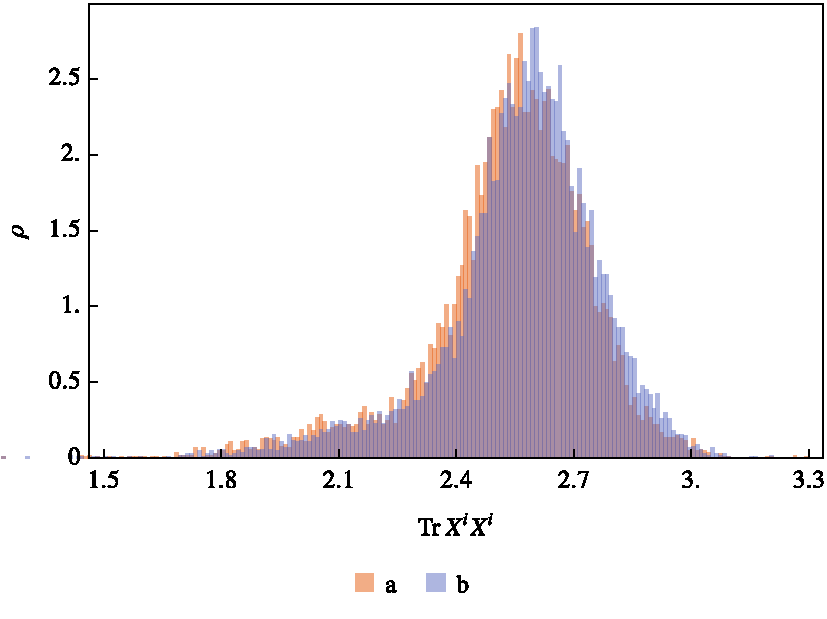
\includegraphics{6-solution-independence}
    \caption{The (time) distribution of $\Tr X^i X^i$ for the same two random states in \cref{fig:6-eig-sol-indep}. Note that the purplish color indicates the region where the distributions overlap.}
    \label{fig:6-solution-independence}
\end{figure}

If one had to guess a form for the distribution of the $x^{i}_{a}$s based on the covariance matrix and on the observation that higher central moments tend to be quite small, the most natural choice would be a multivariable gaussian
\begin{equation}
    p(x) \sim \exp \left( - \mu \sum_{i a} x^{i}_{a} x^{i}_{a} \right)
\end{equation}

However, based on our conventions for the $\mathfrak{su}(N)$ basis (\cref{app:numerical-methods}), the quantity inside the exponential is just $\Tr X^i X^i$ up to a numerical factor.

\begin{figure}[H]
    \centering
    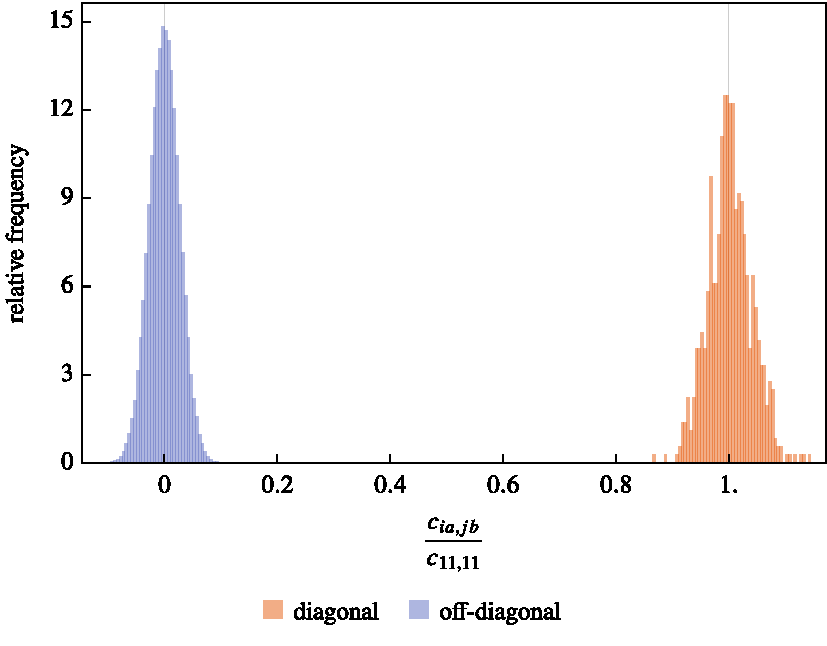
\includegraphics{8-elements-covariance}
    \caption{distribution of the covariance matrix elements (normalized by one of the diagonal values). Note how the spread is around $\epsilon \sim 5\%$.}
    \label{fig:8-elements-covariance}
\end{figure}

Thus, we make the conjecture that the matrices $X^i$ look as if they are identically and independently distributed from a traceless Gaussian Unitary Ensemble (GUE) (see \cref{app:gue}) of rank $N$. In other words, the distribution $p(X)$ of the matrices over long times (and for large $N$, as we will see) is
\begin{equation}\label{eqn:conjecture-distribution}
    p(X) = \left( \frac{\alpha^{(N^2-1)/2}}{Z_{\text{tGUE}}} \right)^K \exp \left( - \frac{\alpha N}{2} \sum_{i} \Tr X^i X^i \right)
\end{equation}
where $Z_{\text{tGUE}}$ is the partition function of traceless GUE, for normalization, and $\alpha$ sets the scale of $X^i$s. Due to (a) the solution independence of various distributions we looked at and (b) the scaling similarity \cref{eqn:scaling-similarity}, it is reasonable to expect that the scale parameter $\alpha$ depends only on $N$ and the scale $\lambda$, or equivalently, the energy $E$ of the solution as follows
\begin{equation}
    \alpha = \alpha(N, E) = \frac{\alpha_N}{\sqrt{E}}
\end{equation}
We can explicitly verify this claim by finding an estimate for $\alpha$ from the simulations and then comparing the random matrix ensemble at this estimated value for $\alpha$ and the simulations themselves. Note that all our simulations have normalized energy $E = 1$, so we need not worry about the dependence of $\alpha$ on $E$: we are directly estimating $\alpha_N$. We consider the following estimates
\begin{enumerate}
    \item[a.] {
        For physical reasons, our primary estimate would come from the distribution of $\Tr X^i X^i$ itself. In particular, both the mean and the variance of this distribution are meaningful quantities to compare to. In essence, we are using a method of moments estimate for the population parameter $\alpha$. It is quite straightforward to show that $\Tr X^i X^i$ follows a gamma distribution (essentially a scaled $\chi^2$-distribution)
        \begin{equation}
            \Tr X^i X^i \sim \Gamma \left( \frac{K(N^2-1)}{2}, \frac{2}{\alpha N} \right)
        \end{equation}
        Thus the mean ($\mu$) and variance ($\sigma^2$) of $\Tr X^i X^i$ are
        \begin{align}
            \mu &= \frac{K(N^2-1)}{\alpha N} \\
            \sigma^2 &= \frac{2K(N^2-1)}{\alpha^2 N^2}
        \end{align}
        Or, for the estimate $\hat{\alpha}_N$, we have (using just the mean $\mu$)
        \begin{align}
            \hat{\alpha}_N = \frac{K(N^2 - 1)}{N \expval{\Tr X^i X^i}}
        \end{align}
    }
    \item[b.] {
        The matrix coefficients $x^{i}_a$ follow a Gaussian distribution. Indeed, this was the first step towards the conjecture. The means, in this case, are not very meaningful since, on both sides, these are very close to zero. However, the variance ($\sigma^2$) can be used to estimate $\alpha$ since
        \begin{equation}
            \sigma^2 = \frac{2}{\alpha N}
        \end{equation}
        from \cref{eqn:conjecture-distribution}. Or, for the estimate
        \begin{equation}
            \hat{\alpha}_N = \frac{2}{N \ \mathrm{Var}\left( x^i_a \right)}
        \end{equation}
    }
    \item[c.] {
        An object simpler than $\Tr X^i X^i$ but is not $\mathrm{SO}(9)$ invariant is $\Tr (X^1)^2$. It is distributed according to
        \begin{equation}
            \Tr (X^1)^2 \sim \Gamma \left( \frac{N^2-1}{2}, \frac{2}{\alpha N}\right)
        \end{equation}
        and so, we have two estimates
        \begin{equation}
            \hat{\alpha}_N = \frac{N^2 - 1}{N \expval{\Tr (X^1)^2}}
        \end{equation}
        from the mean and
        \begin{equation}
            \hat{\alpha}_N = \frac{\sqrt{2(N^2 - 1)}}{N \ \mathrm{SD}\left( \Tr (X^1)^2 \right)}
        \end{equation}
        from the standard deviation.
    }
    \item[d.] {
        A component of the symmetric traceless tensor $\mathfrak{S}$, e.g. $\mathfrak{S}^{1 2} = \Tr X^1 X^2$. The distribution of this object is some generalized gamma distribution. However, to save time, an easier way to estimate $\alpha$ is to numerically generate a large sample of matrices $Y^i$ according to \cref{eqn:conjecture-distribution} with $\alpha = 1$, compute the observable in question: in this case, $\Tr Y^1 Y^2$ and compare ratios of the statistics (e.g., the variance, since the mean is practically zero). The estimate we use here is
        \begin{equation}
            \hat{\alpha}_N = \frac{\mathrm{SD}\left(\Tr Y^1 Y^2\right)}{\mathrm{SD}\left(\Tr X^1 X^2\right)}
        \end{equation}
    }
    \item[e.] {
        The combined eigenvalue distribution: We do not have a closed-form expression for this distribution. It is likely some combination of Hermite polynomials (\cref{app:gue}). But the simpler thing is to generate a large sample $Y^i$ with $\alpha = 1$, compute the eigenvalues $\lambda_Y$ and use
        \begin{equation}
            \hat{\alpha}_N = \frac{\mathrm{Var}\left(\lambda_Y\right)}{\mathrm{Var}\left(\lambda_X\right)}
        \end{equation}
    }
    \end{enumerate}

The result of doing this exercise is summarized in \cref{tab:alpha-val} below. As stated earlier, the primary estimate for $\alpha_N$ comes from the mean of the distribution of $\Tr X^i X^i$. These values of $\alpha_N$ for $N = 3, \ldots, 9$ are shown in \cref{fig:7-alpha} with error bars indicating the dependence on initial conditions. It is interesting to ask whether this $N$-dependence can be obtained from some fundamental considerations about the matrix model and supergravity. At present, we do not have an answer to this. However, the $N$ dependence (for large $N$) can be worked out numerically and turns out to be approximately
\begin{equation}\label{eqn:alpha-fit}
    \alpha_N \approx 2.21 N^{0.529}
\end{equation}
One can see this on a log-log plot of the $\alpha_N$ estimates and the function \cref{eqn:alpha-fit}. This is shown in \cref{fig:7-alpha-fit}.

\begin{table}[H]
    \centering
    \begin{tabular}{ m{0.4cm} m{2.0cm} m{2.0cm} m{2.0cm} m{2.0cm} m{2.0cm} m{1.6cm}} 
    \toprule
    \toprule
    $N$ & $\expval{\Tr X^i X^i}$ & $\sigma\left( x^{i}_a \right)$ & $\expval{\Tr (X^1)^2}$ & $\sigma ( {\Tr (X^1)^2} )$ & $\sigma \left( {\Tr X^1 X^2} \right)$ & $\sigma\left(\lambda\right)$ \\
    \midrule
    3 & \num{15.06(6)}  & \num{14.89(21)} & \num{14.6(25)}  & \num{12.6(21)}   & \num{11.5(22)} & \num{14.85(21)} \\[1.3ex]
    4 & \num{18.78(5)}  & \num{18.91(38)} & \num{18.5(12)}  & \num{16.1(12)}   & \num{16.1(16)} & \num{18.93(38)} \\[1.3ex]
    5 & \num{21.30(6)}  & \num{22.10(26)} & \num{22.36(59)} & \num{20.7(11)}   & \num{19.9(12)} & \num{22.09(26)} \\[1.3ex]
    6 & \num{23.55(17)} & \num{24.53(23)} & \num{24.66(51)} & \num{22.5(9)}  & \num{22.7(12)} & \num{24.52(23)} \\[1.3ex]
    7 & \num{25.52(2)}  & \num{27.14(13)} & \num{27.39(42)} & \num{24.6(16)}   & \num{25.7(14)} & \num{27.16(13)} \\[1.3ex]
    8 & \num{27.53(18)} & \num{29.28(16)} & \num{29.12(33)} & \num{25.6(13)}   & \num{27.9(14)} & \num{29.28(16)} \\[1.3ex]
    9 & \num{29.13(17)} & \num{31.22(21)} & \num{31.17(40)} & \num{27.6(10)} & \num{28.9(15)} & \num{31.22(21)} \\
    \bottomrule
    \bottomrule
    \end{tabular}
\caption{Estimates for $\alpha_N$. The header indicates which statistic was used for the estimate. The statistics used for this table were taken from $\sim 30$ initial conditions for $T = 1000$ with step size $dt = 0.1$}
\label{tab:alpha-val}
\end{table}

\begin{figure}[H]
    \centering
    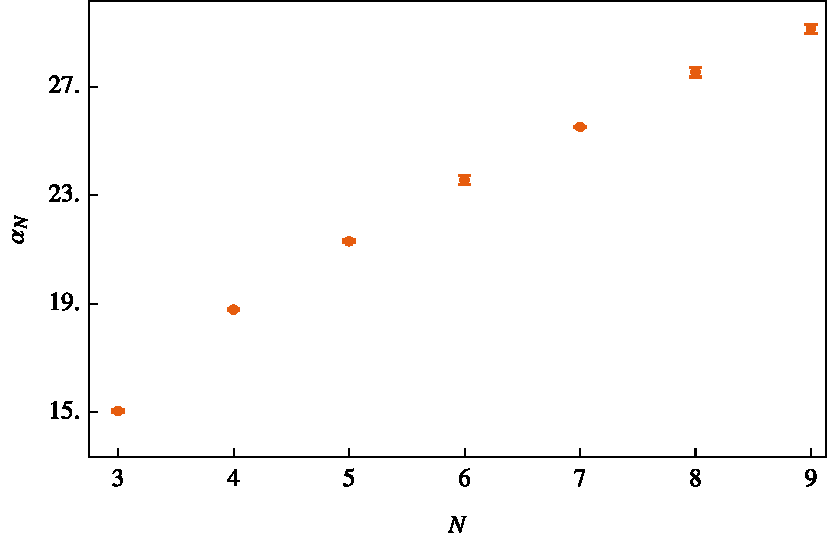
\includegraphics{7-alpha}
    \caption{Primary estimate for $\alpha_N$ (computed using $\expval{\Tr X^i X^i}$) as a function of $N$. Again, error bars indicate variation across initial conditions.} 
    \label{fig:7-alpha}
\end{figure}

\begin{figure}[H]
    \centering
    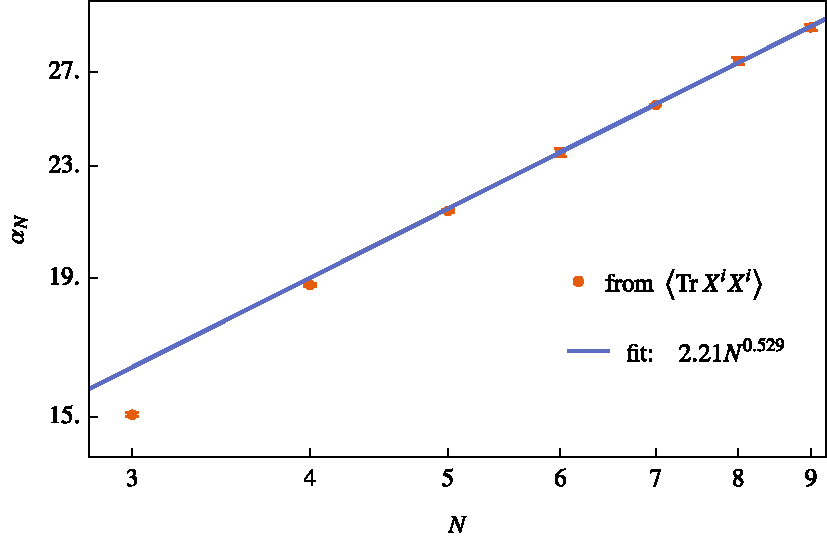
\includegraphics{7-alpha-fit}
    \caption{estimate for $\alpha_N$ (\cref{fig:7-alpha}) in a log-log scale along with a linear fit for the last few points.}
    \label{fig:7-alpha-fit}
\end{figure}

\begin{figure}[H]
    \centering
    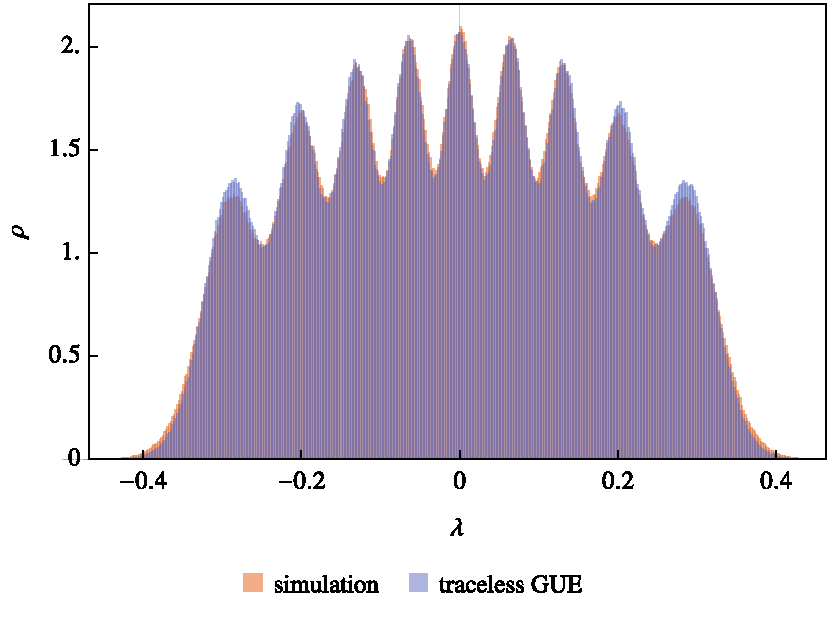
\includegraphics{9-eigenvalues-gue}
    \caption{Eigenvalue distribution at $N = 9$ for matrices obtained through a simulation and the corresponding distribution from traceless GUE, \cref{eqn:conjecture-distribution} with $\alpha$ given in \cref{tab:alpha-val}.}
    \label{fig:9-eigenvalues-gue}
\end{figure}

Having fixed a value of $\alpha$, one can finally ask whether the simulation data is indeed as if it was taken randomly out of a traceless GUE. \cref{fig:9-eigenvalues-gue} shows a plot of the combined eigenvalue distribution for the simulation and for the distribution in \cref{eqn:conjecture-distribution} with $\alpha$ from \cref{tab:alpha-val} (for $N = 9$). The distributions match almost exactly.

Next, we compare the distributions of $\Tr (X^1)^2$ and $\Tr X^i X^i$. In these cases, we know the analytical form of the distributions (gamma distributions). \cref{fig:9-trX1sq-gue,fig:9-trXsq-gue} show the comparison. One observes that as we sum more of the $\Tr X^i X^i$, there is a significant departure from random matrix behavior. Limited evidence suggests that this is a finite $N$ phenomenon, and as one approaches larger $N$, these deviations disappear, but more work needs to be done to verify these claims. In particular, we need to access larger values of $N$. 

\section{Departure from random matrix behavior}

Interestingly, the deviation from traceless GUE for $\Tr X^i X^i$ cannot be attributed to sampling error or looking at an odd observable alone. This is because the time statistics of relatively high order of $\Tr X^i X^i$ still show universal, initial condition-independent behavior. However, these higher-order solution-independent statistics differ significantly from their tGUE counterparts. 

\begin{figure}[H]
    \centering
    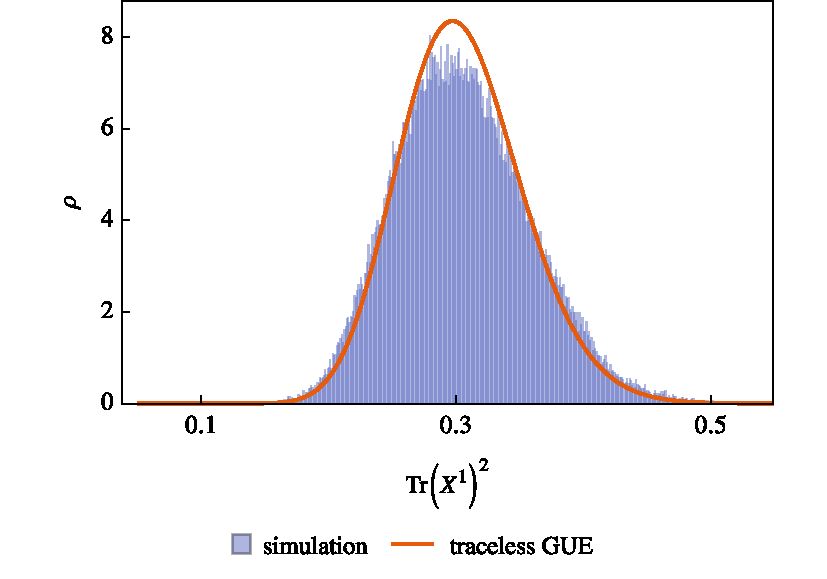
\includegraphics{9-trX1sq-gue}
    \caption{distribution of $\Tr (X^1)^2$ compared for the simulation data and the distribution from \cref{eqn:conjecture-distribution} (a gamma distribution) with the same parameters as in \cref{fig:9-eigenvalues-gue}.}
    \label{fig:9-trX1sq-gue}
\end{figure}

Let us quickly define the statistics we look at. For simplicity, let us denote the $n^\mathrm{th}$ central moment by $c_n$. Mean ($c_1$) and variance ($c_2$) are as usual, but we look at two new statistics
\begin{enumerate}
    \item[a.] {
        \textbf{Skewness ($b_1$)}: This is related to the third central moment $c_3$ as
        \begin{equation}
            b_1 = \frac{c_3}{(c_2)^{3/2}}
        \end{equation}
    }
    \item[b.] {
        \textbf{Kurtosis ($b_2$)}: Related to the fourth central moment $c_4$
        \begin{equation}
            b_2 = \frac{c_4}{(c_2)^{2}}
        \end{equation}
    }
\end{enumerate}

\cref{tab:deviations-from-random} summarizes these statistics for three sets of simulation data starting at random initial conditions and lastly for traceless GUE (\cref{eqn:conjecture-distribution}) with $\alpha$ from \cref{tab:alpha-val}. Note that even higher order statistics like $b_1$ and $b_2$ are consistent across multiple initial conditions but depart significantly from traceless GUE.

\begin{figure}[H]
    \centering
    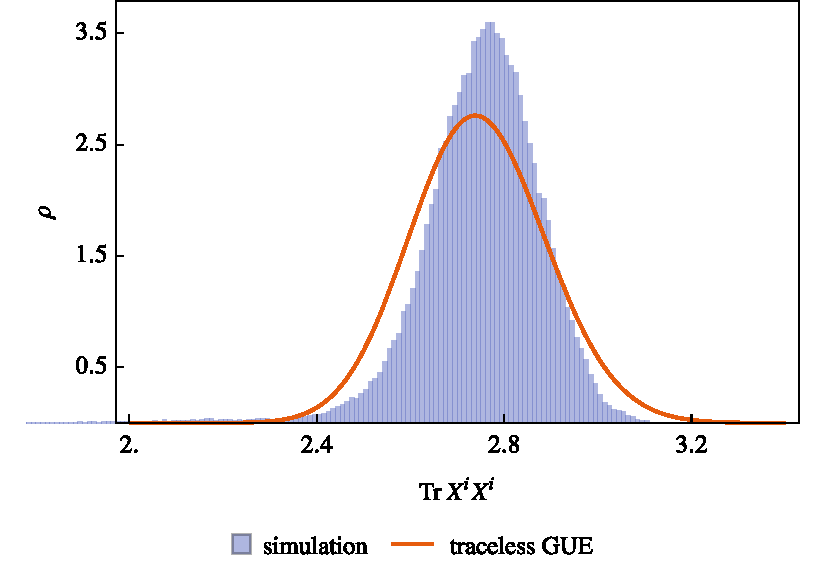
\includegraphics{9-trXsq-gue}
    \caption{Distribution of $\Tr X^i X^i$. Note how even though the means agree, the higher moments differ quite a bit (e.g., the simulation data is much more skewed than the gamma distribution).}
    \label{fig:9-trXsq-gue}
\end{figure}

\begin{table}[H]
\centering
    \begin{tabular}{ m{2.0cm} m{2.0cm} m{2.0cm} m{2.0cm} m{1.5cm}} 
    \toprule
    \toprule
    \textbf{Type} & \textbf{Mean} & \textbf{Standard Deviation} & \textbf{Skewness} & \textbf{Kurtosis} \\
    \midrule
    Random 1 & 2.742 & 0.1367 & -1.62  & 15.89 \\[1.3ex]
    Random 2 & 2.746 & 0.1376 & -1.733 & 15.86 \\[1.3ex]
    Random 3 & 2.74  & 0.1417 & -1.59  & 14.23 \\[1.3ex]
    Traceless GUE & 2.746 & 0.1446 & 0.1208 & 3.067 \\[1.3ex]
    \bottomrule
    \bottomrule
    \end{tabular}
\caption{Higher order statistics for $\Tr X^i X^i$ at $N = 9$ for random states and traceless GUE}
\label{tab:deviations-from-random}
\end{table}

These could be indications of significant higher-order correlations between the matrix variables that are not taken into account by the simple form of \cref{eqn:conjecture-distribution}. More work is needed to show that these correlations become unimportant at larger $N$.